\section{Preliminaries}
\label{sec:preliminaries}

In the remainder of the paper, we endeavor to solve a synthesis problem for
assume-guarantee contracts involving infinite theories.  Formally, an
implementation is a set of valid initial states $I$ and transition relation $T$ that implements the contract.  In this section, we introduce the necessary formal machinery to talk about {\em realizations} of an assume-guarantee contract.

\subsection{Example}
As an illustrative example, consider the contract specified in
Figure~\ref{fg:example}. The component to be designed consists of two
inputs, $x$ and $y$ and one output $z$. If we restrict our example to the case
of integer arithmetic, we can see that the contract assumes that the inputs will
never have the same value, and requires that the component's output is a boolean
whose value depends on the comparison of the values of $x$ and $y$.

\begin{figure}[H]
	\centering
	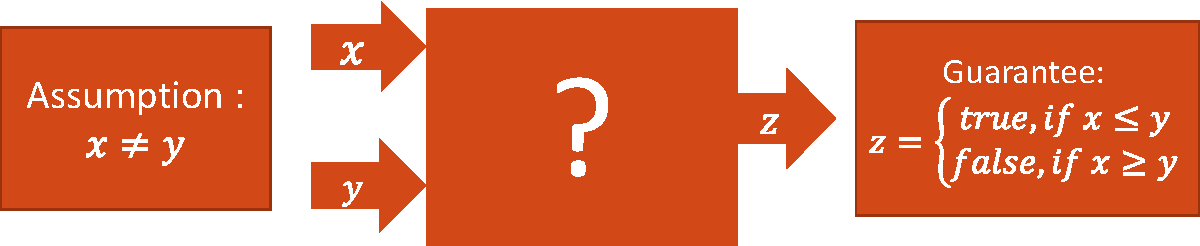
\includegraphics[width=0.45\textwidth,height=\textheight,keepaspectratio]{real1-crop}    	
	\caption{Example of a realizable contract}
	\label{fg:example}
\end{figure}


One can easily prove that an implementation able to satisfy the contract is
possible. The same though does not apply in the case where we omit the
assumption from our original contract. Given no constraints over the values that the inputs can take, we have a case where the implementation may
behave in an inconsistent manner regarding the value of $z$, thus making the
violation of the guarantees possible. In the first case, the contract is realizable, but in the second, we
cannot find an implementation that can provide us with an output that satisfies
the contract guarantees, for any valid input. These contracts are considered to
be unrealizable.

\subsection{Formal Definitions}
We use the types $state$ and $inputs$ to describe a state
and the set of inputs in the system, respectively. We define a
\textit{transition system} as a pair $(I,T)$, where $I$ is the set of initial states, of type $state \rightarrow
bool$ and $T$ is the transition relation, of type $state \rightarrow inputs
\rightarrow state \rightarrow bool$. 

A contract in this context is defined by its
\textit{assumptions} and \textit{guarantees}. The \textit{assumptions} $A$
impose constraints over the inputs, while the \textit{guarantees} are
further decomposed into the pair $(G_I,G_T)$ with $G_I$ describing the
valid initial states for the system, and $G_T$ specifying the new states to which
the system may transition, given a specific state and input. Note that
we do not necessarily
expect that a contract would be defined over all variables in the
transition system,
but we do not make any distinction between internal state variables
and outputs in the formalism.  This way, we can use state variables to, in some cases, simplify statements of guarantees.

Given the above, we expressed realizability as follows. A state $s$ is
\textit{viable} if, starting from $s$, the transition system is capable of continuously responding to
incoming valid inputs. Alternatively, $s$ is $viable$ if the transitional
guarantee $G_T$ infinitely holds, given valid inputs. As such,
viability is defined coinductively:
\begin{equation}
\label{eq:viable}
Viable(s) = \forall i. A(s,i) \Rightarrow \exists s'. G_{T}(s,i,s') \wedge
Viable(s')
\end{equation}
Using the definition of $viable$, a
contract is $realizable$ if and only if
\begin{equation}
\label{eq:realizable}
 \exists s.~ G_I(s) \land Viable(s).
\end{equation}

To use this coinductive formula in a model checking framework, we had to further
massage the definition into one that resembles the principle of
\textit{k-induction}. As such, the base step of the induction ensures that
given a state, $G_T$ can keep responding to valid inputs for at least $n$ steps
in the future. We call this state \textit{finitely viable}, written
$Viable_{n}(s)$:
\begin{multline}
\label{ml:fv}
		\forall i_1. A(s,i_1) \Rightarrow \exists s_1. G_T(s,i_1,s_1) \wedge~ \\
			\hspace{+0.5cm} \forall i_2. A(s_1,i_2) \Rightarrow \exists s_2.
			 G_T(s_1,i_2,s_2) \wedge \ldots \wedge~ \\
			 \hspace{+1.5cm} \forall i_n. A(s_{n-1},i_n) \Rightarrow \exists s_n. G_T(s_{n-1},i_n,s_n)
	\end{multline}

On the other hand, the inductive step checks whether a path starting from a
finitely viable state can be further extended one-step. We call states that
build such paths \textit{extendable}, written $Extend_{n}(s)$:
	\begin{multline}
	\label{ml:extendable}
		\forall i_1,s_1,\ldots,i_n,s_n. \\
		\hspace{-2cm} A(s,i_1) \wedge G_T(s,i_1,s_1) \wedge \ldots \wedge \\
		A(s_{n-1}, i_n) \wedge G_T(s_{n-1},i_n,s_n) \Rightarrow \\
		\hspace{+2cm} \forall i. A(s_n,i) \Rightarrow \exists s'. G_T(s_n,i,s')
	\end{multline}
	
Considering these underapproximations, the algorithm is split into two separate
checks. For the \textit{BaseCheck}, we ensure that there exists an initial
finitely viable state,
\begin{equation}
\label{bcheck}
BaseCheck(n) = \exists s. G_I(s) \wedge Viable_n(s)
\end{equation}
while the \textit{ExtendCheck} tries to prove that all
valid states are extendable.
\begin{equation}
\label{eq:echeck}
ExtendCheck(n) = \forall s. Extend_n(s)
\end{equation}
Due to the definition of finite viability containing $2n$
quantifier alternations, we can not practically use \textit{BaseCheck} as the
current SMT solvers struggle solving formulas of such structure. Therefore we
finally proposed a simplified version of \textit{BaseCheck}, which essentially
tries to prove that all initial states are extendable for any $k \leq n$.
\begin{equation}
\label{eq:sbcheck}
BaseCheck'(n) = \forall k \leq n. (\forall s. G_I(s)
	  	\Rightarrow Extend_k(s))
\end{equation}

Even though the simplified definition is more simple for an SMT solver to
process, it comes with a cost, as it introduces cases of realizable contracts
that are considered to be unrealizable from the algorithm. To the extent of our
experiments, such a case has yet to be met, as it inherently requires the user
to purposely define contracts of such behavior.

